%% This is file `elsarticle-template-1-num.tex',
%%
%% Copyright 2009 Elsevier Ltd
%%
%% This file is part of the 'Elsarticle Bundle'.
%% ---------------------------------------------
%%
%% It may be distributed under the conditions of the LaTeX Project Public
%% License, either version 1.2 of this license or (at your option) any
%% later version.  The latest version of this license is in
%%    http://www.latex-project.org/lppl.txt
%% and version 1.2 or later is part of all distributions of LaTeX
%% version 1999/12/01 or later.
%%
%% Template article for Elsevier's document class `elsarticle'
%% with numbered style bibliographic references
%%
%% $Id: elsarticle-template-1-num.tex 149 2009-10-08 05:01:15Z rishi $
%% $URL: http://lenova.river-valley.com/svn/elsbst/trunk/elsarticle-template-1-num.tex $
%%
\documentclass[12pt]{elsarticle}

\makeatletter
\def\ps@pprintTitle{%
   \let\@oddhead\@empty
   \let\@evenhead\@empty
   \let\@oddfoot\@oddfoot
   \let\@evenfoot\@evenfoot
}
\makeatother

%% Use the option review to obtain double line spacing
%% \documentclass[preprint,review,12pt]{elsarticle}

%% Use the options 1p,twocolumn; 3p; 3p,twocolumn; 5p; or 5p,twocolumn
%% for a journal layout:
%% \documentclass[final,1p,times]{elsarticle}
%% \documentclass[final,1p,times,twocolumn]{elsarticle}
%% \documentclass[final,3p,times]{elsarticle}
%% \documentclass[final,3p,times,twocolumn]{elsarticle}
%% \documentclass[final,5p,times]{elsarticle}
%% \documentclass[final,5p,times,twocolumn]{elsarticle}

\usepackage{hyperref} 
%% The graphicx package provides the includegraphics command.
\usepackage{graphicx}
%% The amssymb package provides various useful mathematical symbols
\usepackage{amssymb}
%% The amsthm package provides extended theorem environments
%% \usepackage{amsthm}
\usepackage{caption}
\usepackage{subcaption}
\usepackage{cite}

%% The lineno packages adds line numbers. Start line numbering with
%% \begin{linenumbers}, end it with \end{linenumbers}. Or switch it on
%% for the whole article with \linenumbers after \end{frontmatter}.
%\usepackage{lineno}

%% natbib.sty is loaded by default. However, natbib options can be
%% provided with \biboptions{...} command. Following options are
%% valid:

%%   round  -  round parentheses are used (default)
%%   square -  square brackets are used   [option]
%%   curly  -  curly braces are used      {option}
%%   angle  -  angle brackets are used    <option>
%%   semicolon  -  multiple citations separated by semi-colon
%%   colon  - same as semicolon, an earlier confusion
%%   comma  -  separated by comma
%%   numbers-  selects numerical citations
%%   super  -  numerical citations as superscripts
%%   sort   -  sorts multiple citations according to order in ref. list
%%   sort&compress   -  like sort, but also compresses numerical citations
%%   compress - compresses without sorting
%%
%% \biboptions{comma,round}

% \biboptions{}

%\journal{}

\graphicspath{{./}{Documents}}

\begin{document}

\begin{frontmatter}

%% Title, authors and addresses

\title{After Segmental Autonomy: Assessing Conflict and Service Proliferation in Mali's Autonomous Region}

%% use the tnoteref command within \title for footnotes;
%% use the tnotetext command for the associated footnote;
%% use the fnref command within \author or \address for footnotes;
%% use the fntext command for the associated footnote;
%% use the corref command within \author for corresponding author footnotes;
%% use the cortext command for the associated footnote;
%% use the ead command for the email address,
%% and the form \ead[url] for the home page:
%%
%% \title{Title\tnoteref{label1}}
%% \tnotetext[label1]{}
%% \author{Name\corref{cor1}\fnref{label2}}
%% \ead{email address}
%% \ead[url]{home page}
%% \fntext[label2]{}
%% \cortext[cor1]{}
%% \address{Address\fnref{label3}}
%% \fntext[label3]{}


%% use optional labels to link authors explicitly to addresses:
%% \author[label1,label2]{<author name>}
%% \address[label1]{<address>}
%% \address[label2]{<address>}

\author{Thomas J. Brailey}

\address{University of California, San Diego}

\begin{abstract}
%% Text of abstract
When ethnic groups are granted regional autonomy by the state’s national government, what do we expect to see? Existing literature posits that segmental autonomy, by allowing minority groups to act independently of the central government, can lead to a decrease in conflict in ethnically diverse societies. That said, this literature is highly contested and few quantitative studies exist to support these claims. Further, existing literature on segmental autonomy focuses almost exclusively on conflict, failing to address other possible outcomes of granting autonomy such as regional economic output, services, and development in the autonomous region. In 2000, the Mali government granted autonomy to the Tuareg minority population along the north-east border with Niger. Using conflict and health-services data three years prior to, and three years post, autonomy, this paper utilizes geographic information systems (GIS) in order to map conflict rates and health service proliferation in and around the Tuareg's autonomous region in Mali. 
\end{abstract}

\begin{keyword}
Segmental Autonomy \sep Power-Sharing \sep GIS
%% keywords here, in the form: keyword \sep keyword

%% MSC codes here, in the form: \MSC code \sep code
%% or \MSC[2008] code \sep code (2000 is the default)

\end{keyword}

\end{frontmatter}

%%
%% Start line numbering here if you want
%%
%\linenumbers

%% main text
\section{Overview}

Prior to achieving autonomy in 2000, the Tuareg, a regional ethnic group located in north eastern Mali and Niger, had been pressuring the Mali government to decentralize decision-making and funding allocations. Though the Mali government were concerned that the Tuareg might push for a complete secession from the state, they refused to grant the Tuareg people regional autonomy\footnote{For the purposes of this paper, I use the terms regional and segmental autonomy interchangeably.}. The increase in political pressure by the Tuareg culminated in a coup d’état in 1991 against authoritarian leader Moussa Traoré\footnote{Humphreys, 2005}. The following year saw the introduction of peace accords granting the Tuareg some level of regional autonomy. Though intended to abate tensions between the central government and the ethnic groups in Mali, the peace accords were not fully implemented until 1999 when the first Tuareg regional elections were held\footnote{Keita, 1998}. Prior to the regional elections, rates of politically-motivated conflict between the Tuareg, the central government, and other minority ethnic populations, remained high. In the years following the \textit{de facto} implementation of regional autonomy, conflict rates and fatalities appeared to decrease. The Ethnic Power-Relations Atlas (EPR) anecdotally remarks that following regional autonomy in the north east, conflict rates decreased within the Tuareg region\footnote{Vogt et al., 2015}.

Existing literature on the efficacy of segmental autonomy is often limited to a conflict lens, and the empirical methods produce mixed results\footnote{Brown, 2009; Cederman et al., 2015; Mattes and Savun, 2009}. Studies that suggest that segmental autonomy is effective in reducing conflict raise several caveats regarding their methodology, including the presence of potential endogeneity, interaction effects with other power-sharing provisions, and other country-specific confounders. Moreover, little interest has been taken in mapping the location of these conflicts, so while overall conflicts in a country may be decreasing, we cannot determine if segmental autonomy has a positive effect in reducing conflict \textit{within} the autonomous area. Similarly, research on the impacts of segmental autonomy outside of the context of war are sparse and produce equally dubious results\footnote{Duncan, 2007}. 

This paper seeks to understand, using geographic information systems (GIS) methods, to what extent conflict rates decreased in Mali, and whether this decrease is spatially significant. A second objective of this paper is to understand the proliferation of health services in the newly autonomous region. Using health service proliferation as a proxy for development, I seek to understand whether there are any other spatial relationships between the implementation of segmental autonomy and the political or economic success of the autonomous region. In answering these questions, we can better understand the impact of segmental autonomy on ethnically diverse states from a spatial perspective. Given the lack of geospatial, temporal, studies on autonomy, any findings from my analyses will give some unique insight into the impact of states granting autonomy to ethnic minorities. Given the existing literature and case study analyses, my first hypothesis is that following the implementation of regional autonomy, the autonomous region will experience a decrease in conflict in the years following. Similarly, I expect to see a proliferation in the establishment of health services in the autonomous region, assuming that the Tuareg minority had considerably more fiscal and policy manoeuvrability after 2000.

\section{Mapping Conflict and Service Proliferation}
In answering my first question--whether the implementation of segmental autonomy leads to a decrease in the frequency and intensity of conflict--I utilize data from the Armed Conflict Location and Event Data Project (ACLED)\footnote{Raleigh et al., 2010}. This database records all conflict reported in local and international news reports, and contains information on non-deadly conflicts, the type of conflict, and the actors involved. For my second hypothesis, I utilize data from the Global Healthsites Mapping Project (GHMP), an open-source, real-time mapping of all health facilities across the world\footnote{Hostettler, 2018}. Both ACLED and GHMP have high accuracy coordinates of conflict and health site location respectively. These XY values can be mapped in ArcGIS. The Ethnic Power-Relations data project has geocoded data for ethnic groups around the world\footnote{Vogt et al., 2015}. I use R to subset and then join data from the standard EPR dataset to the GeoEPR dataset, mapping the location of the Tuareg minority in Mali and using this layer as a mask and an independent variable when running my models\footnote{Replication code for this project--and others--can be found on my Github account at \href{https://github.com/tjbrailey/RegionalAutonomyGIS}{https://github.com/tjbrailey/RegionalAutonomyGIS}}. Lastly, I use the Database of Global Administrative Areas (GADM) to map the extent of Africa, Mali, and the administrative boundaries therein. Given the nature of my models, I keep all of my point data and shapefiles in a WGS 1984 projection\footnote{GADM, 2019}. 

\subsection{Conflict}
Upon subsetting the data to include information three years prior to and three years after the Tuareg region was granted segmental autonomy, we find forty-one unique conflicts with fatalities ranging from zero to forty. Given the sparseness of the data, one cannot reasonably run spatial models beyond simple summary statistics. As such, I utilize ArcGIS's zonal statistics function--and the Tuareg shapefile as a mask--to generate several summary tables from which I can calculate additional statistics using the field calculator tool. Table 1 shows the culmination of this model and produces some interesting initial findings. We see that, three years prior to the Tuareg being granted regional autonomy, fatalities in the Tuareg region accounted for roughly sixty percent of the total fatalities in Mali. Post-autonomy, the total number of conflicts dropped from eighty-nine to thirty-six, and the percentage of fatalities in the autonomous region as a percentage of total fatalities in Mali dropped to eight percent. Figure 1 provides a geo-visualization of the information in Table 1.

\begin{table}
    \tiny
\begin{center}
    \resizebox{\textwidth}{!}{
\begin{tabular}{l c c c c c}
\hline
 \\
 & Autonomy & Total Fatalities & Fatalities in Autonomous Region & \% of Fatalities in AR \\
 \\
  \hline
 \\
    & Pre-Autonomy & 89 & 57 & 64.04 \\ 
 \\
    & Post-Autonomy & 36 & 3 & 8.33 \\ 
 \\
   \hline
\end{tabular}}
\caption{Fatalities in Mali (1997 - 2003)}
\end{center}
\end{table}

While these results are interesting, one must recognize the potential pitfalls with the data. Firstly, analyzing conflict undoubtedly raises issues of endogeneity, reverse causality, and spuriousness. Perhaps some exogenous shock occurred, unrelated to the provision of autonomy, that drastically reduced conflict rates in the state. While outside of the scope of this paper, it is my intention to run these models again across polities with country fixed-effects and other potential explanatory variables such as regional quality of life, ethnic fractionalization, and so on. Secondly, while the work of ACLED is laudable, I intend to run these models again using data from the Peace Research Institute Oslo (PRIO) and the Social Conflict Analysis Database (SCAD) to ensure my results account for all known conflicts in the region. In any case, this initial visualization provides some support to the claim that, at least in Mali-Tuareg case, the introduction of segmental autonomy provisions may indeed reduce conflict both within the autonomous region and within the state as a whole. 

\begin{figure}[h]
\centering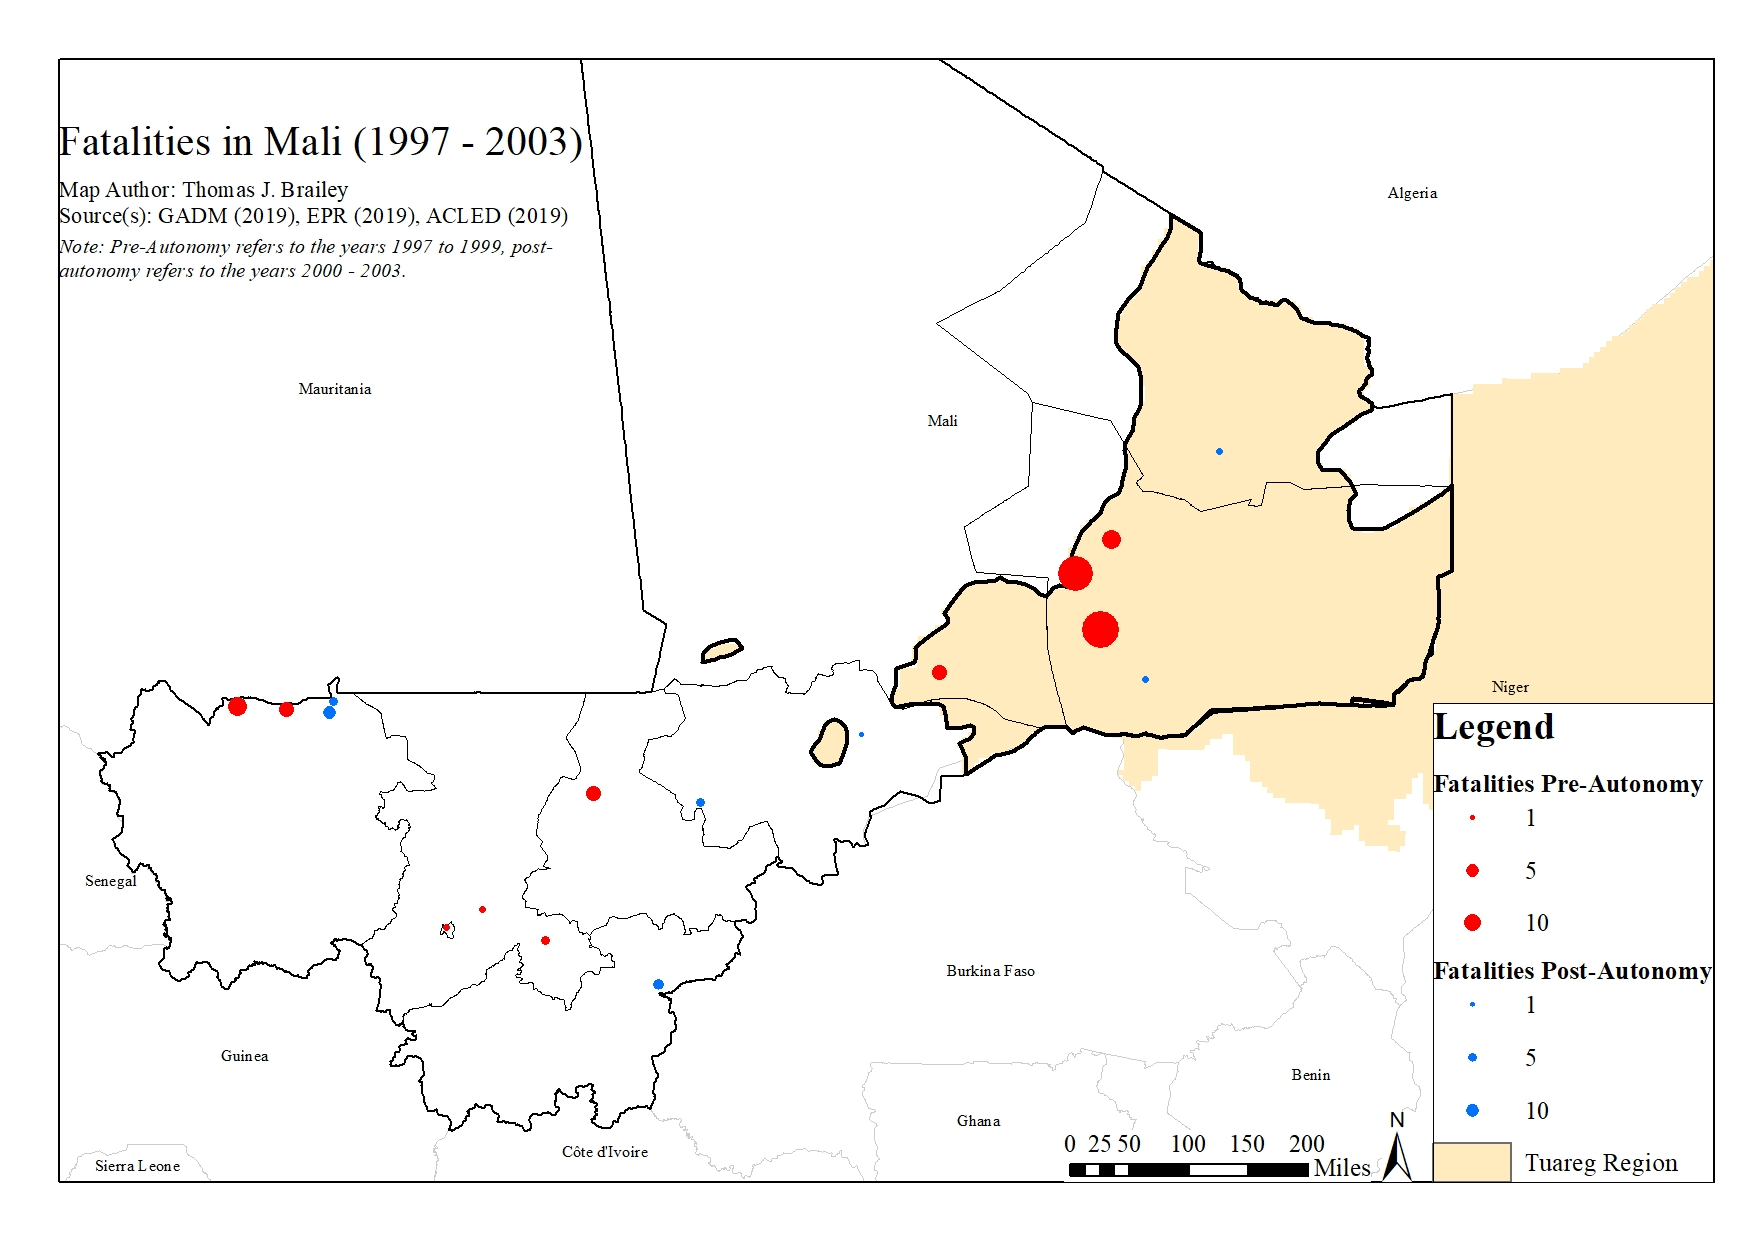
\includegraphics[width=\textwidth,height=\textheight,keepaspectratio]{tjbrailey_final_project_map_conf.jpg}
\caption{Georeferenced Conflict Fatalities In Mali (1997 - 2003)}
\end{figure}

\subsection{Health Services}
Given that there are far more observations for health services in Mali, I am able to use more intricate statistical models to understand the relationship between the implementation of regional autonomy and the proliferation of services. The models and results will be covered in more depth in the next section, but I start by mapping the location of each health service and, by selecting by attributes, I create two separate layers for pre-autonomy and post-autonomy. While simply mapping the XY coordinates worked well in visualizing the conflict data, few inferences can be made with the health service data. As such, I utilize ArcGIS's kernel density function which calculates a magnitude-per-unit area from the health site point features using a kernel function to fit a smoothly tapered surface to each point. This function assumes planar distances, given that I am not working with projected shapefiles or rasters. Figures 2 and 3 show the change in the proliferation of health services pre- and post-autonomy.

Anecdotally, we see the largest proliferation of health sites occur in Bamako, the capital city of Mali, and along the more populous regions in the south of the country. As expected, we see very little to no health sites being established in the more northern regions, as these are locations deep within the Sahara Desert. These patterns hold steady before and after the provision of autonomy in the state. More interestingly, we see an increase in the density of health sites--as shown by the darker blue regions--between the two time periods. We also see more health sites being developed in the south-eastern portion of the Tuareg region. To reiterate, these first three figures are simple visualizations that do not imply statistical significance, rather, they are designed to better understand the spatial relationship between the provision of autonomy, conflict, and the provision of services; relationships that have yet to be explored through a GIS lens. The next section will address the issue of statistical significance regarding the health sites data using both ordinary least squares regression (OLS) and geographically weighted regression (GWR).

\begin{figure}
\centering
\begin{subfigure}{.8\textwidth}
  \centering
  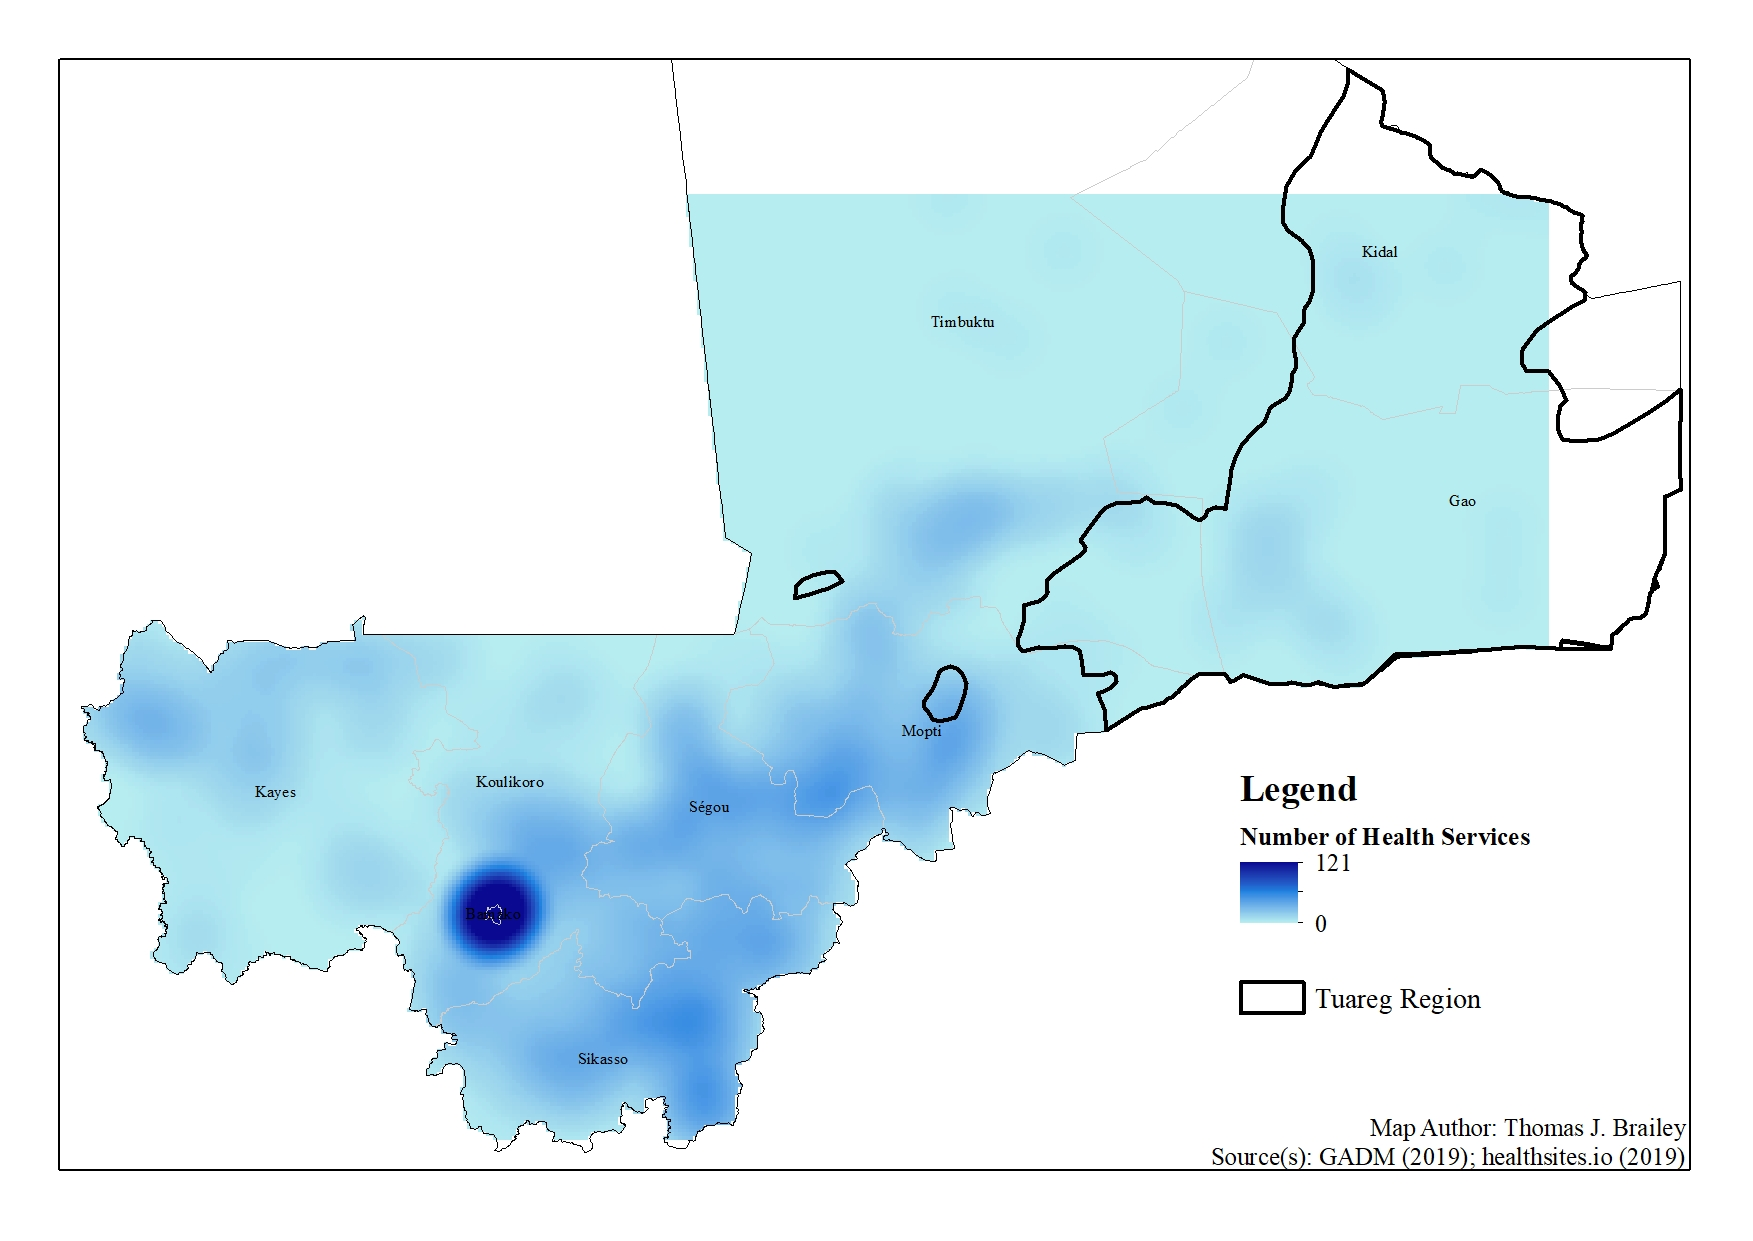
\includegraphics[width=1\linewidth]{tjbrailey_final_project_map_health_kernel_pre.jpg}
\end{subfigure}%
\caption{Kernel Density Pre-Autonomy}
\end{figure}
\begin{figure}
\centering
\begin{subfigure}{.8\textwidth}
  \centering
  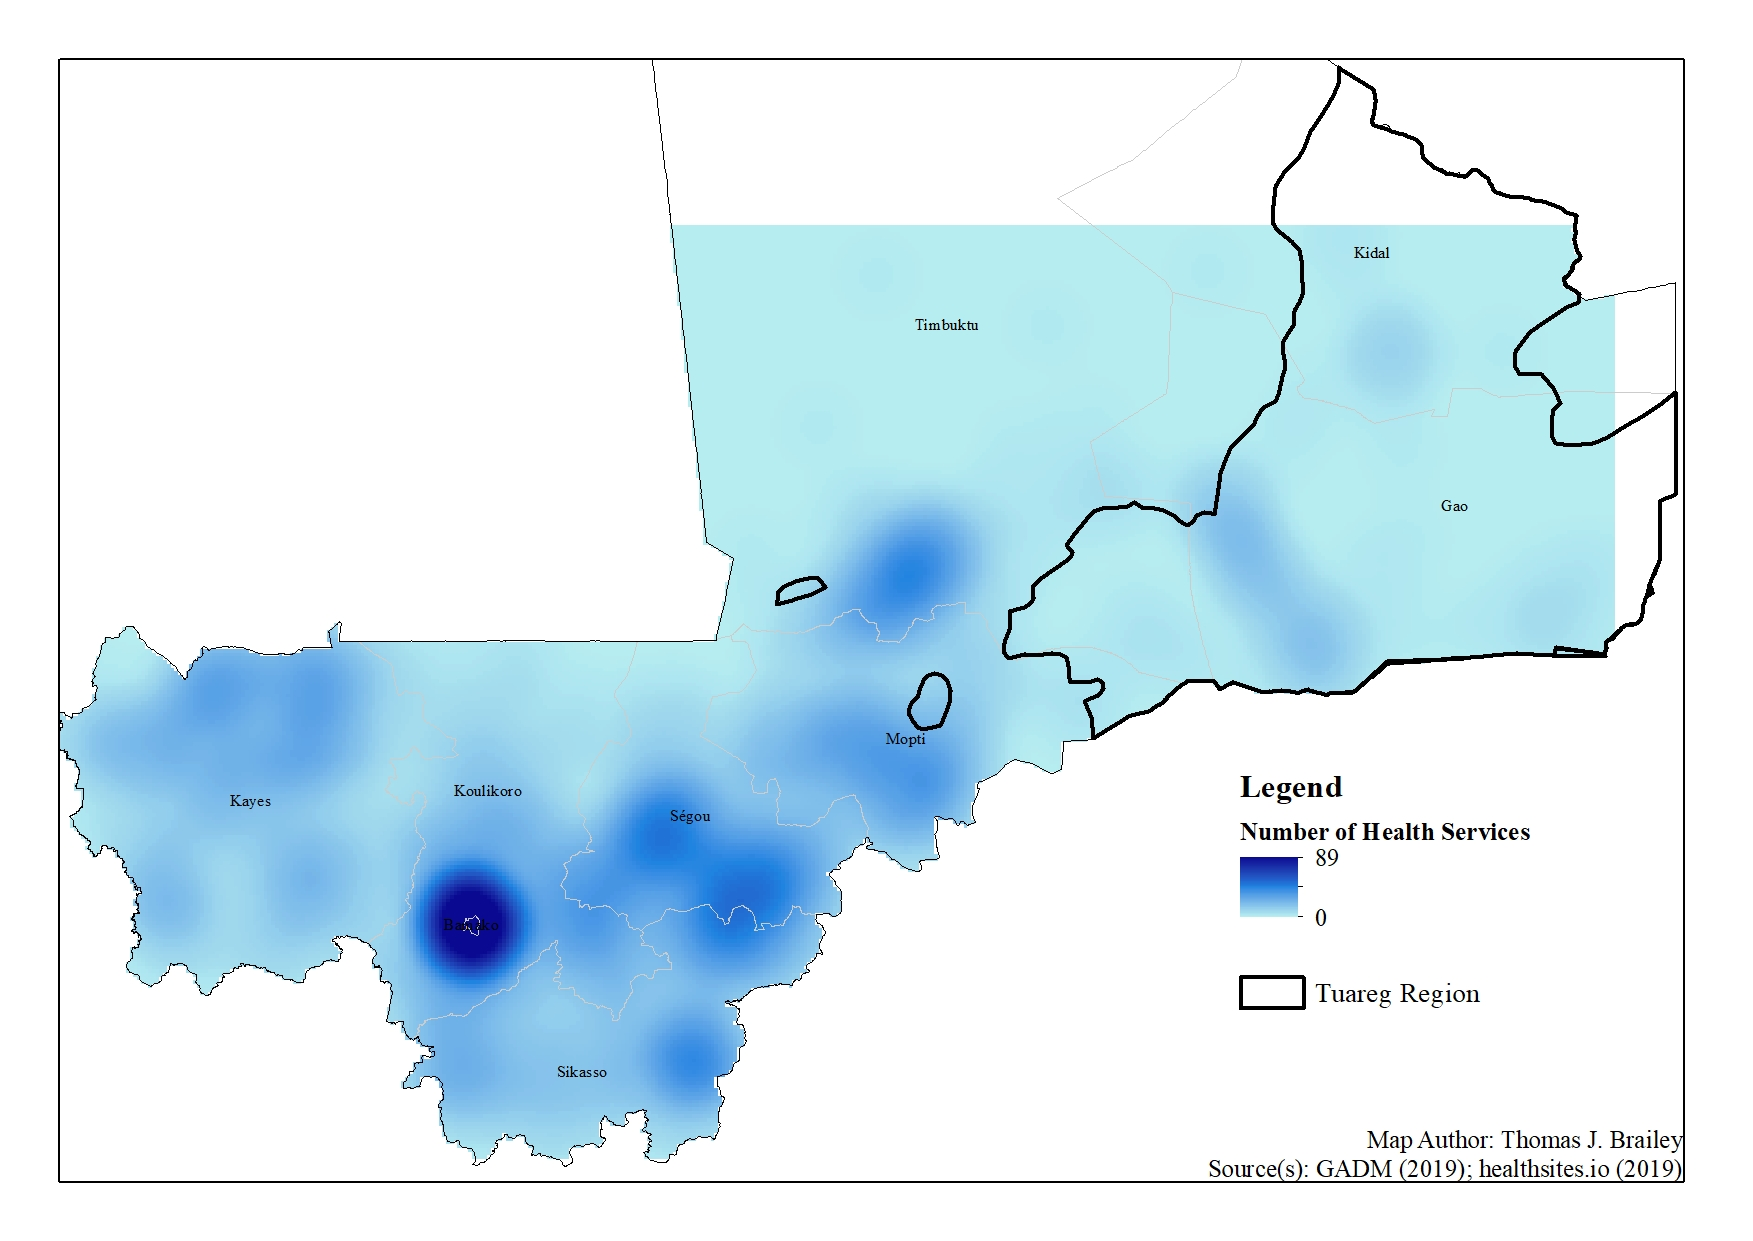
\includegraphics[width=1\linewidth]{tjbrailey_final_project_map_health_kernel_post.jpg}
\end{subfigure}%
\caption{Kernel Density Post-Autonomy}
\end{figure}

\section{Statistical Models}
In order to ascertain whether the relationship between the proliferation of health services and the provision of regional autonomy, I start by running an ordinary least squares regression which is described using the estimation equation below. 

\begin{equation}
\label{eq:emc}
Health Sites = \beta_0 + \beta_1 AR + \beta_2 Pop + \epsilon
\end{equation}

Here, \textit{AR} is a binary variable for whether the gridcell falls within the autonomous region or not and \textit{Pop} is the sum of the population in that gridcell. Unlike the kernel density models, I calculate the dependent variable \textit{HealthSites} to be the difference in the number of health sites built pre- and post-autonomy. Thus, if the value of the difference variable is larger than zero, then we know that more health sites have been built in the post-autonomy period. Likewise, if the value is negative, there were more health sites built in the pre-autonomy period. I then regress this value on whether that area, irrespective of time, is the autonomous region or not. For robustness, I control for the Mali population\footnote{Linard et al., 2012} \footnote{Though I had intended to include, and spent much time searching for, additional controls such as ethnic fractionalization, regional GDP, and quality of life, such fine-grain spatial measurements are seemingly difficult to obtain and verify for sub-Saharan states.}. 

These calculations are made by first converting a population raster for Mali into a polygon shapefile, and then spatially joining the shapefile to a fishnet which contains the number of health sites both pre- and post-autonomy aggregated to 0.5 by 0.5 decimal degree grids. The final fishnet, then, contains, in each grid cell, data on the number of health sites before autonomy, after autonomy, the change in the proliferation of health sites, whether that region falls within the autonomous boundaries, and the total population living in that grid cell. 

\begin{table}
    \small
\begin{center}
    \resizebox{\textwidth}{!}{
\begin{tabular}{|l|l|l|l|l|l|l|l|l|}
\hline
Variable & Coefficient & SE & t-Statistic & Probability & Robust\_SE & Robust\_t & Robust\_Pr & VIF \\ 
\hline 
Intercept & 0.313325 & 0.260954 & 1.200694 & 0.231623 & 0.235747 & 1.329077 & 0.185698 & --------          \\
Autonomous Region & 0.334476 & 0.638009 & 0.524250 & 0.600828 & 0.411816 & 0.812198 & 0.417861 & 1.032720  \\
Population & 0.000000 & 0.000002 & 0.075852 & 0.939620 & 0.000002 & 0.088022 & 0.929957 & 1.032720         \\
\hline
\end{tabular}}
\end{center}
\caption{OLS Results}
\end{table}

\subsection{Results}
Figure 4 shows the estimated coefficient of the difference in the proliferation of health sites before and after the Tuareg's autonomy in 2000. While the map of the OLS regression seems to confirm my initial hypothesis, in a bid to understand whether the results have an spatial relationship, I include both the OLS report (Table 2) as well as a spatial autocorrelation report (Table 3). Two findings emerge. Firstly, neither independent variable exerts a statistically significant effect on the dependent variable, the reasons behind which will be explored in the last section. Secondly, given that the Moran's I statistic shows a small p-value and a positive z-score, I reject part of the null hypothesis and conclude that the spatial distribution of my variables are more spatially clustered than would be expected if underlying spatial processes were random. Moreover, the results suggest that the OLS model underestimates the standard errors. Though my results are not statistically significant, the results from the Moran's I provide impetus to run a localized model, a geographically weighted regression, in order to account for Type I error and potential spatial nonstationarity.

\begin{table}
    \small
\begin{center}
    %\resizebox{\textwidth}{!}{
\begin{tabular}{|l|l|}
\hline
\multicolumn{2}{|c|}{Global Moran's I Summary}  \\
\hline
Moran's Index:          &           0.081769    \\
Expected Index:         &	        -0.006098   \\ 
Variance:	            &           0.001262    \\
z-score:	            &           2.473060    \\
p-value:     	        &           0.013396    \\  
\hline
\end{tabular}%}
\end{center}
\caption{Spatial Autocorrelation Report}
\label{table:coefficients}
\end{table}

\begin{figure}[ht]
\centering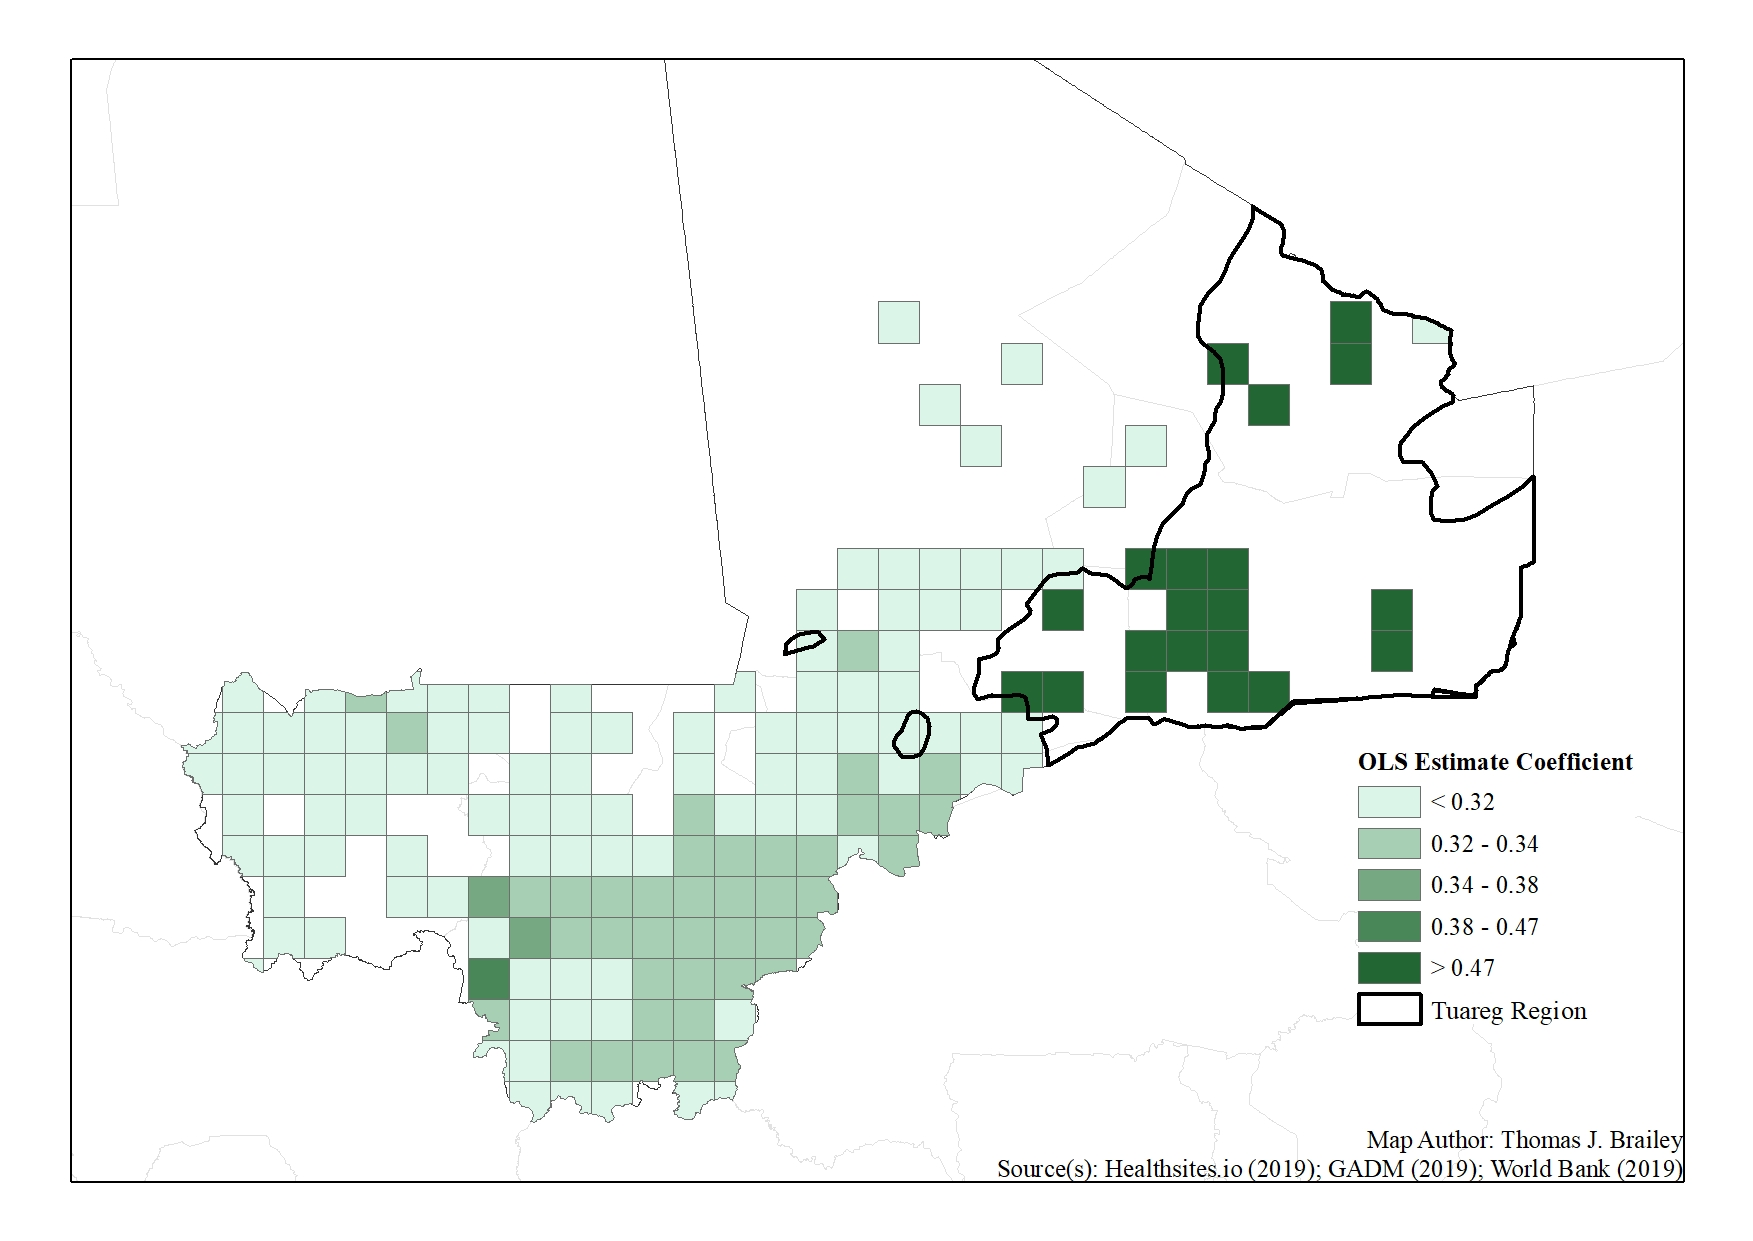
\includegraphics[width=\textwidth,height=\textheight,keepaspectratio]{tjbrailey_final_project_map_health_ols.jpg}
\caption{Ordinary Least Squares Model}
\end{figure}

\subsection{Localized and Robust Models}
Using the same fishnet data and variables as before, I run GWR with a fixed kernel and AICc bandwidth, and manually calculate a t-statistic for each observation. The coefficient results for the presence of the autonomous region are more conservative compared to the OLS and, again, none of the observations are statistically significant.  As such, I have not included the mapped GWR results given that it does not serve to better explain the results from the OLS output. 

A final note on the statistical models: because ArcGIS's OLS report suggests that the residuals for the dependent and independent variables are not normally distributed, I use R to run a robust linear model on the logged values of these variables. Even when accounting for residual distribution, we do not find statistical significance for either independent variable\footnote{A table of results for the robust linear model can be found in the appendix.}.  

\section{Summary of Findings}
This paper began by presenting a basic map of the number of fatalities in Mali pre- and post-autonomy. Though only anecdotal, we see a sharp decrease in the number of fatalities and the number of conflicts both in the autonomous region and throughout Mali in the post-2000 period. Future research should both expand the time periods before and after segmental autonomy is granted in a state, and offer comparative country models in order to deduce whether it is in fact the provision of autonomy which is reducing conflict. 

I then run kernel densities on my larger dataset on health site proliferation and find similar anecdotal evidence that, upon being granted autonomy and representation in government, the Tuareg region sees an increase in the proliferation of health services within its boundaries. Though my kernel density models suggested that there appears to be a greater proliferation in health services in the autonomous region after being granted segmental autonomy, OLS, GWR, and robust models suggest that this pattern is more likely to be random chance. 

While, for the purposes of this paper, we must accept the null hypothesis that there is no statistically significant relationship between the implementation of segmental autonomy provisions and the proliferation of health services, there may be a few potential explanations for these results. Firstly, we are limited to one proxy for services which has a relatively low number of observations. Secondly, we are limited by the data to study a six year period within one country. Lastly, given that there exist relatively few regionally-focused datasets for sub-Saharan Africa, we are missing potentially important explanatory variables and measurements. Future studies should focus on expanding and deepening these fine-grain data on regional economic output, ethnic fractionalization, and the like. One final point, though outside the scope of this paper, it would be beneficial to conduct a geospatial difference-in-difference model to compare conflict rates (and other dependent variables) between Mali and Niger, both in which the Tuareg minority group are present. This would be an interesting study as we could compare the effects of implementing autonomy (Mali) to avoiding decentralization (Niger) with two contiguous, relatively well-matched, states. 

\subsection{Conclusion}
When a state is granted segmental autonomy, what do we expect to see? I have shown, using geospatial data on Mali and the Tuareg ethnic population therein, that there is anecdotal evidence supporting the claim that autonomy is beneficial for the autonomous region and the state as a whole. Though my results do not suggest statistical significance, this paper presents a methodological framework by which, given more data across a larger time period, we can better understand the potential impacts of implementing segmental autonomy in ethnically diverse states.

%% The Appendices part is started with the command \appendix;
%% appendix sections are then done as normal sections
%% \appendix

%% \section{}
%% \label{}

%% References
%%
%% Following citation commands can be used in the body text:
%% Usage of \cite is as follows:
%%   \cite{key}          ==>>  [#]
%%   \cite[chap. 2]{key} ==>>  [#, chap. 2]
%%   \citet{key}         ==>>  Author [#]

%% References with bibTeX database:

%% New version of the num-names style

\nocite{*}
\bibliographystyle{elsarticle-num}
\bibliography{reg_aut_mali}

\section{Appendix}
\begin{table}[htp]
\begin{center}
\begin{tabular}{l c}
\hline
 & Model 1 \\
\hline
(Intercept)         & $-0.55$  \\
                    & $(0.85)$ \\
Autonomous Region   & $0.50$   \\
                    & $(0.43)$ \\
Logged Population   & $0.08$   \\
                    & $(0.09)$ \\
\hline
R$^2$               & $0.00$   \\
Adj. R$^2$          & $-0.01$  \\
Num. obs.           & $165$    \\
RMSE                & $2.63$   \\
\hline
\multicolumn{2}{l}{\scriptsize{$^{***}p<0.001$; $^{**}p<0.01$; $^{*}p<0.05$}}
\end{tabular}
\caption{Robust Linear Model with Logged Values}
\end{center}
\end{table}
%% Authors are advised to submit their bibtex database files. They are
%% requested to list a bibtex style file in the manuscript if they do
%% not want to use model1-num-names.bst.

%% References without bibTeX database:



%% \bibitem must have the following form:
%%   \bibitem{key}...
%%




\end{document}

%%
%% End of file `elsarticle-template-1-num.tex'.